
\documentclass{article}
\usepackage{fontspec}
\setmainfont{Times New Roman}
\setmonofont{Menlo}

\usepackage{amsmath,amssymb,booktabs,longtable,array,calc,graphicx,xcolor,hyperref}
\usepackage[margin=25mm]{geometry}
\hypersetup{colorlinks=true,linkcolor=blue,urlcolor=blue}
\setlength{\parindent}{0pt}
\setlength{\parskip}{6pt}
\providecommand{\tightlist}{\setlength{\itemsep}{0pt}\setlength{\parskip}{0pt}}
\providecommand{\pandocbounded}[1]{\begin{center}\resizebox{0.96\linewidth}{!}{#1}\end{center}}
\newcounter{none}
\makeatletter
\define@key{Gin}{alt}{}
\makeatother

\begin{document}
\section{Preliminary Numerical Study of Gray-Cat Metastable Interfaces,
Weak C Readout, and Strong D Observation Selection in a Closed Phase
System
v1}\label{preliminary-numerical-study-of-gray-cat-metastable-interfaces-weak-c-readout-and-strong-d-observation-selection-in-a-closed-phase-system-v1}

\textbf{Date:} 2026-07-14\\
\textbf{Author:} Noriaki Kihara\\
\textbf{Series:} Wave Information Readout / preliminary numerical study
of A/B allocation metastability and observation selection in a closed
system\\
\textbf{Version DOI:} 10.5281/zenodo.21353209\\
\textbf{Concept DOI:} 10.5281/zenodo.21353208

\begin{center}\rule{0.5\linewidth}{0.5pt}\end{center}

\subsection{0. Conclusion}\label{conclusion}

This paper summarizes a preliminary numerical experiment in which the
white-cat state \texttt{A} and the black-cat state \texttt{B} are
represented by closed-system complex amplitudes

\[
a,\quad b
\]

and read through

\[
p_A=|a|^2,\qquad p_B=|b|^2,
\]

\[
Q=p_A+p_B,\qquad S=p_A-p_B.
\]

The white-cat, black-cat, and gray-cat terminology is used here only as
a metaphor for A/B allocation states. It is not a claim to reproduce the
standard Schrodinger-cat thought experiment itself.

The experiment confirms the following points.

\begin{verbatim}
1. In the AB two-body system alone, a gray eigen phase,
   a gray metastable phase, and a natural selection phase were separated.
2. Under weak C readout, a window existed in which the gray metastable
   phase could be read without selecting one side.
3. Under strong D observation, the gray metastable phase was selected
   into either the white-cat or black-cat allocation.
4. In the gray eigen phase, the gray allocation was kept even under
   strong D observation.
5. No-D controls did not show equivalent white/black selection, so the
   selection could be separated as D-induced in the tested cases.
\end{verbatim}

Thus the observed classification is:

\begin{verbatim}
gray metastable phase:
  weak readout reads it as gray;
  strong observation selects white or black.

gray eigen phase:
  weak readout reads it as gray;
  strong observation keeps it gray.
\end{verbatim}

When the result is white-selected,

\[
S \simeq +1,\qquad p_A\simeq 1,\qquad p_B\simeq 0.
\]

When the result is black-selected,

\[
S \simeq -1,\qquad p_A\simeq 0,\qquad p_B\simeq 1.
\]

This should be read as an almost one-sided relocation of the A/B
allocation, not as the appearance of two cats. The closed quantity

\[
Q=p_A+p_B
\]

is preserved.

\begin{center}\rule{0.5\linewidth}{0.5pt}\end{center}

\subsection{1. Background and Aim}\label{background-and-aim}

The wave-information-readout series has studied whether position-like,
momentum-like, energy-like, and acceleration-like quantities can be
constructed from closed complex phase relations and interference
readouts without assuming a background space in advance.

The preceding acceleration-basis and localization-exchange experiment
studied how localization and effective harmonic order are redistributed
by an AB interaction based on an exchange-interference scattering
matrix.

This paper moves that line of work to the selection of an A/B allocation
state.

The question is:

\begin{verbatim}
Is a mixed white-cat A and black-cat B allocation merely an unselected state,
or can it be held as a gray-cat eigen state?

How does the state respond to weak C readout and strong D observation?
\end{verbatim}

The experiment is divided into four stages.

\begin{verbatim}
Stage 1:
  Search for gray eigen, gray metastable, and natural selection phases
  in the AB two-body system alone.

Stage 2:
  Test whether weak C readout can read the gray metastable phase without
  selecting one side.

Stage 3:
  Test whether strong D observation selects the gray metastable phase
  into white or black.

Stage 4:
  Sweep the D observation start step and D gain to read the selection boundary.
\end{verbatim}

\subsection{1.1 State Transition
Diagram}\label{state-transition-diagram}

The three representative paths are shown below along the AB, ABC, and
ABCD stages.

\begin{figure}
\centering
\pandocbounded{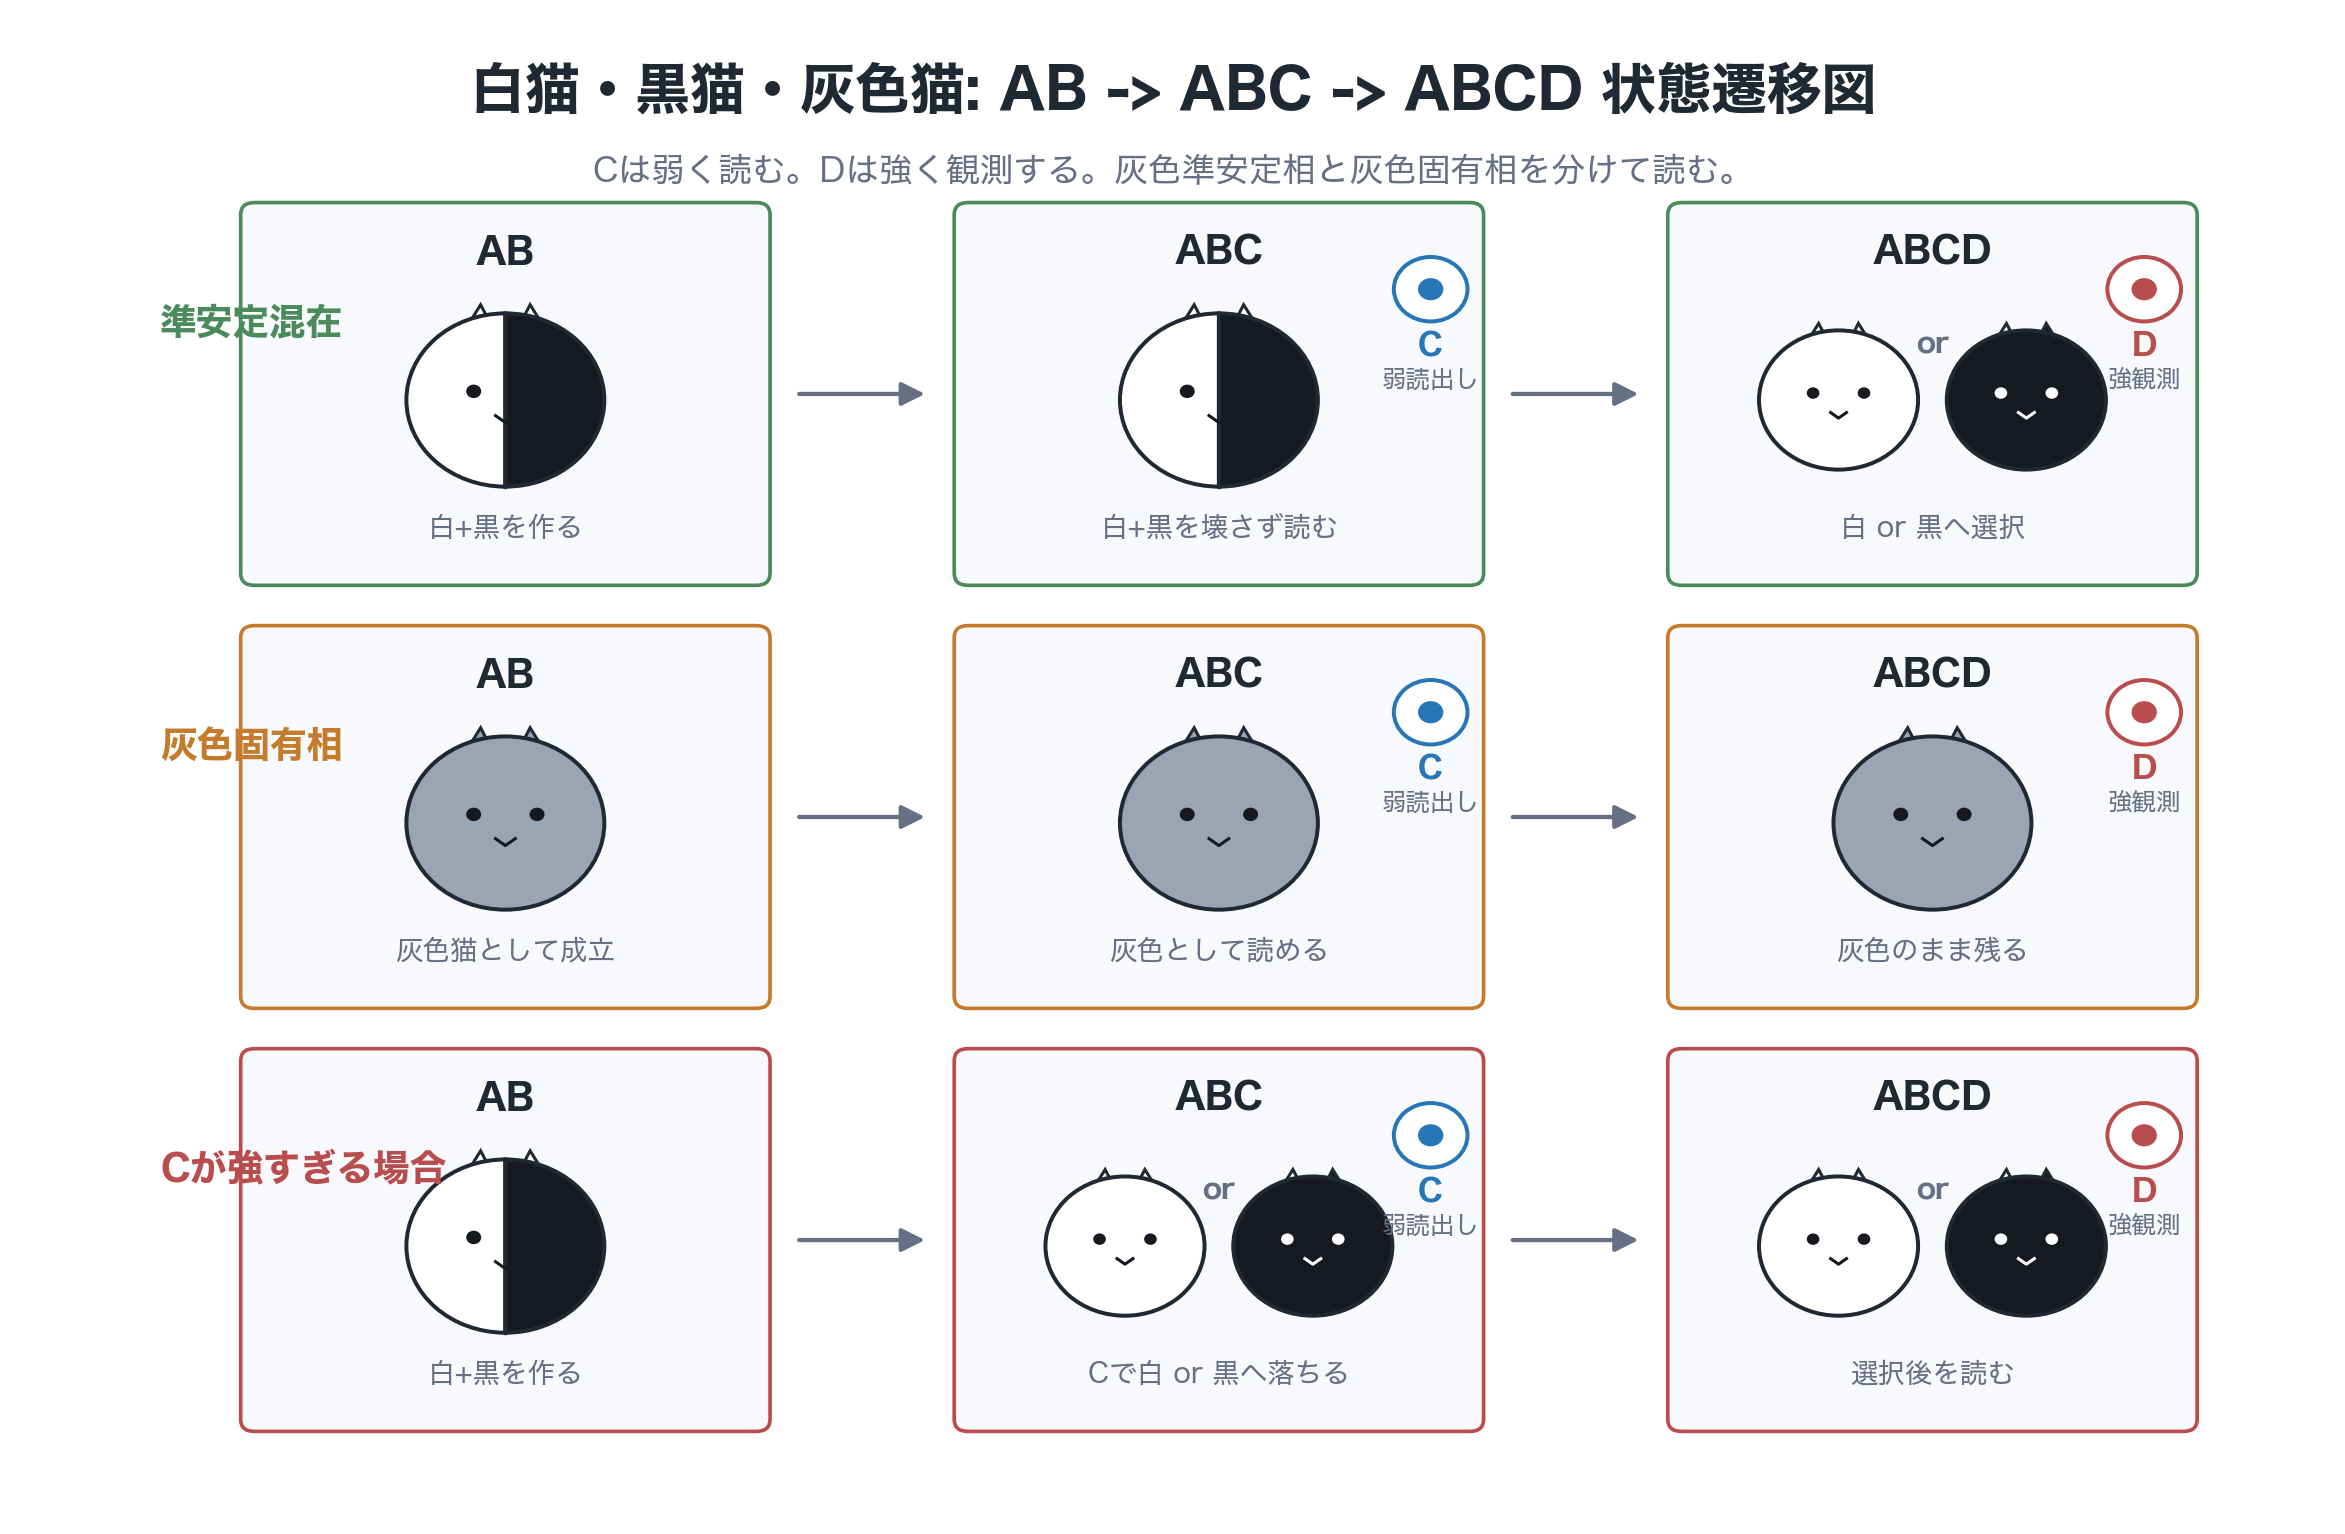
\includegraphics[keepaspectratio,alt={White, black, and gray cat AB-ABC-ABCD state transition diagram}]{gray_cat_state_transition_figures_v1/gray_cat_ab_abc_abcd_three_scenarios_v1.png}}
\caption{White, black, and gray cat AB-ABC-ABCD state transition
diagram}
\end{figure}

The upper path shows a metastable white+black mixture prepared in AB,
weakly read by C, and selected into white or black by strong D
observation.

The middle path shows a gray eigen phase already formed at the AB stage
and kept gray under both weak C readout and strong D observation.

The lower path shows the case in which C is too strong and selection
into white or black already occurs at the ABC stage.

\subsection{1.2 Observed-Value Transition
Diagram}\label{observed-value-transition-diagram}

The same three paths are also shown using the computed values of
\texttt{p\_A}, \texttt{p\_B}, and \texttt{S}.

\begin{figure}
\centering
\pandocbounded{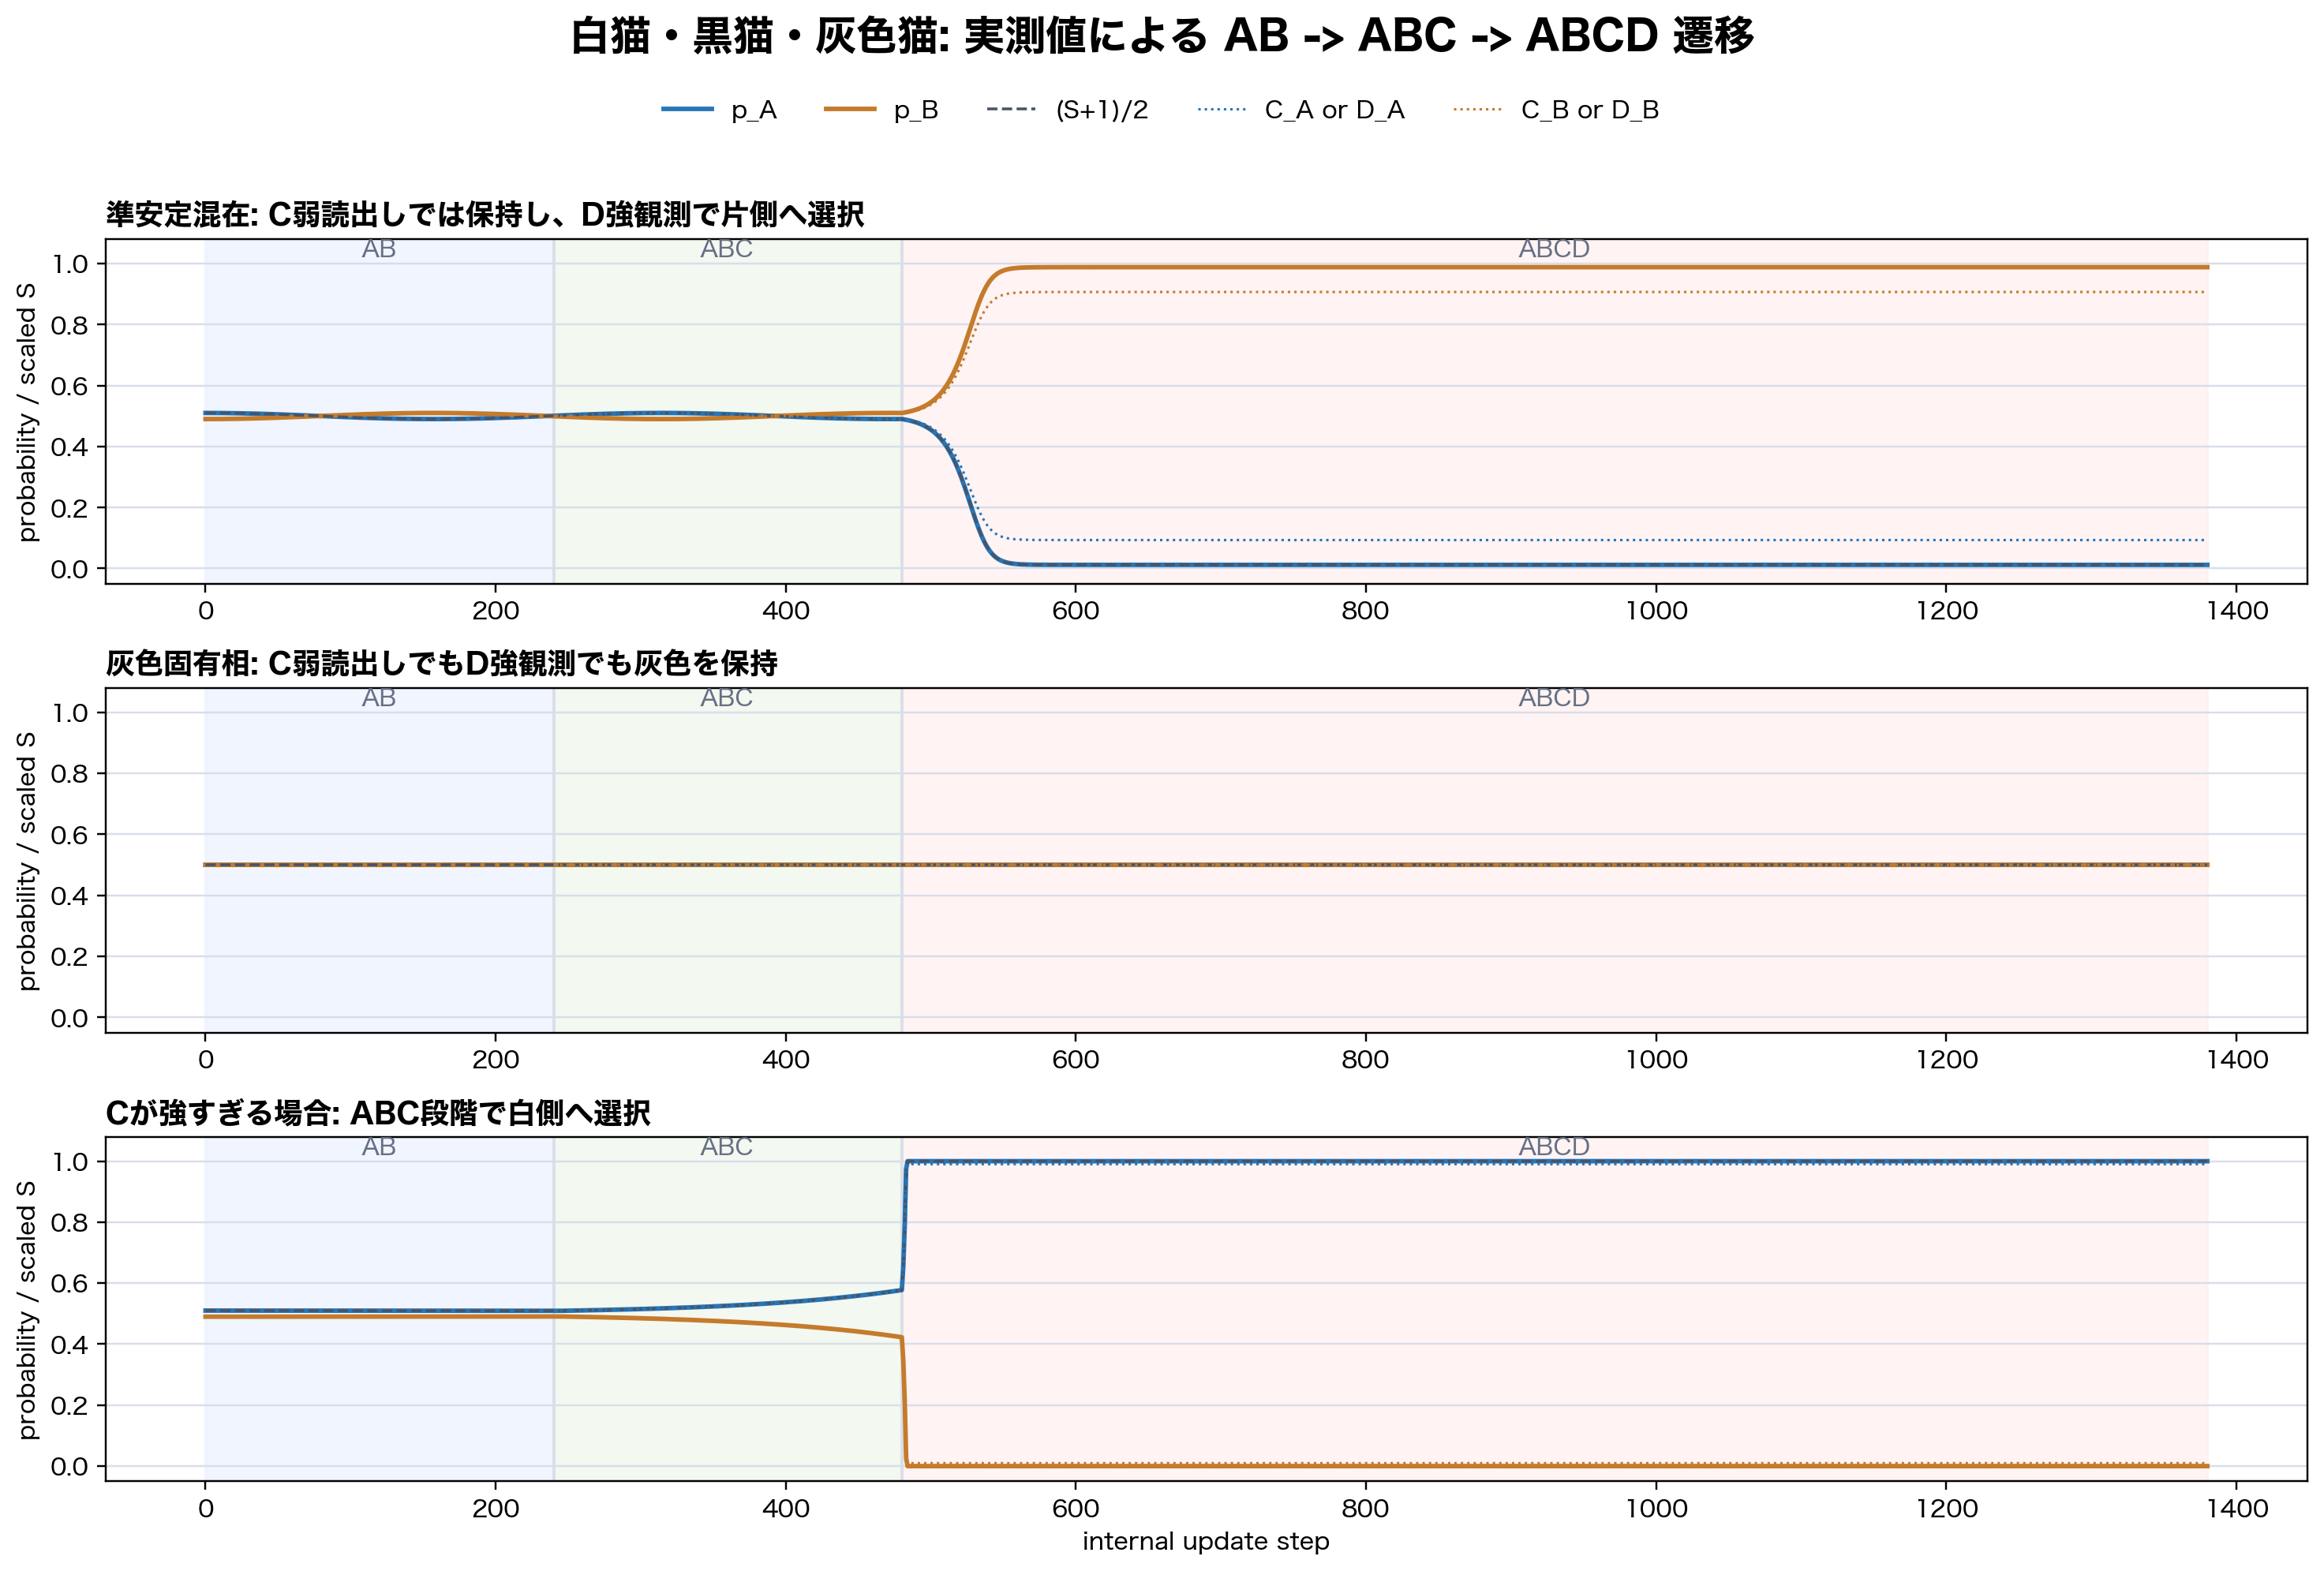
\includegraphics[keepaspectratio,alt={Observed-value transition of white, black, and gray cat states}]{gray_cat_observed_value_transition_figures_v1/gray_cat_ab_abc_abcd_observed_values_three_scenarios_v1.png}}
\caption{Observed-value transition of white, black, and gray cat states}
\end{figure}

The solid curves are the internal values \texttt{p\_A} and
\texttt{p\_B}. The dashed curve is the selection order variable mapped
to the same vertical axis as

\[
\frac{S+1}{2}.
\]

The dotted curves represent the C readout in the ABC interval and the D
readout in the ABCD interval.

\begin{center}\rule{0.5\linewidth}{0.5pt}\end{center}

\subsection{2. Variables and Phase
Classification}\label{variables-and-phase-classification}

\subsection{2.1 A/B Allocation}\label{ab-allocation}

The A/B allocation is read as

\[
p_A=|a|^2,\qquad p_B=|b|^2.
\]

The closed quantity is

\[
Q=p_A+p_B.
\]

The A/B selection order variable is

\[
S=p_A-p_B.
\]

Then

\[
p_A=\frac{1+S}{2},
\qquad
p_B=\frac{1-S}{2}.
\]

\subsection{2.2 White, Black, and Gray Cat
Readouts}\label{white-black-and-gray-cat-readouts}

{\def\LTcaptype{none} % do not increment counter
\begin{longtable}[]{@{}lll@{}}
\toprule\noalign{}
State & Numerical guide & Readout \\
\midrule\noalign{}
\endhead
\bottomrule\noalign{}
\endlastfoot
white cat & \texttt{S≈+1} & \texttt{p\_A≈1}, \texttt{p\_B≈0} \\
black cat & \texttt{S≈-1} & \texttt{p\_A≈0}, \texttt{p\_B≈1} \\
gray cat & \texttt{S≈0} & \texttt{p\_A≈0.5}, \texttt{p\_B≈0.5} \\
\end{longtable}
}

\subsection{2.3 Phase Classification}\label{phase-classification}

For the AB-only evolution, the phases are classified as follows.

\begin{verbatim}
gray_eigen:
  S_mean ≈ 0
  S_amp ≈ 0
  S_drift ≈ 0

gray_metastable:
  S_mean ≈ 0
  0 < S_amp < S_gray_limit
  S_drift ≈ 0

natural_selection:
  S -> +1 or S -> -1 even without C or D.

large_oscillation:
  S oscillates strongly and a clear A/B bias appears.
\end{verbatim}

The main targets of this paper are \texttt{gray\_metastable} and
\texttt{gray\_eigen}.

\begin{center}\rule{0.5\linewidth}{0.5pt}\end{center}

\subsection{3. Model}\label{model}

\subsection{3.1 AB Exchange Interaction}\label{ab-exchange-interaction}

The minimal AB exchange map is

\[
\begin{pmatrix}
a_{k+1}\\
b_{k+1}
\end{pmatrix}
=
U_\epsilon
\begin{pmatrix}
a_k\\
b_k
\end{pmatrix},
\]

\[
U_\epsilon
=
\begin{pmatrix}
\cos\epsilon & i\sin\epsilon\\
i\sin\epsilon & \cos\epsilon
\end{pmatrix}.
\]

A weak restoring term or a weak nonlinear term may be added to test
closed-system stability. However, conditions that naturally select one
side without C or D are not counted as observation-induced selection.

\subsection{3.2 Weak C Readout}\label{weak-c-readout}

C is an internal readout wave that weakly reads the A/B allocation. The
visibility is

\[
v_C=\frac{g_C}{g_C+\kappa_C}.
\]

Then

\[
S_C=v_CS,
\]

\[
C_A=\frac{1+S_C}{2},
\qquad
C_B=\frac{1-S_C}{2}.
\]

C is used to search for a window where the A/B allocation can be read
without selecting one side.

\subsection{3.3 Strong D Observation}\label{strong-d-observation}

D is a strong observation map that amplifies the currently read
direction of \texttt{S}. Its visibility is

\[
v_D=\frac{g_D}{g_D+\kappa_D},
\]

and

\[
S_D=v_DS.
\]

The D backaction is implemented as

\[
S_{k+1}
=
S_k
+
G_D S_D(1-S_k^2),
\]

where \texttt{G\_D} is the D gain.

For the same D start state, a no-D control is run in parallel. If the
no-D control also falls into the same white-cat or black-cat selection,
the result is not counted as D-induced selection.

\begin{center}\rule{0.5\linewidth}{0.5pt}\end{center}

\subsection{4. Stage 1: AB Metastable Interface
Search}\label{stage-1-ab-metastable-interface-search}

\subsection{4.1 Conditions}\label{conditions}

\begin{verbatim}
C = off
D = off
steps = 4096
S_gray_limit = 0.05
selection_limit = 0.95
\end{verbatim}

The main swept parameters were:

\begin{verbatim}
epsilon_values = (0.0, 1e-05, 3e-05, 0.0001, 0.0003, 0.001, 0.003, 0.01)
stability_gain_values = (-0.01, -0.002, 0.0, 0.002, 0.01)
\end{verbatim}

\subsection{4.2 Results}\label{results}

{\def\LTcaptype{none} % do not increment counter
\begin{longtable}[]{@{}lr@{}}
\toprule\noalign{}
phase & count \\
\midrule\noalign{}
\endhead
\bottomrule\noalign{}
\endlastfoot
\texttt{gray\_eigen} & \texttt{1248} \\
\texttt{gray\_metastable} & \texttt{733} \\
\texttt{large\_oscillation} & \texttt{470} \\
\texttt{natural\_selection} & \texttt{1070} \\
\texttt{unstable\_or\_drifting} & \texttt{2079} \\
\end{longtable}
}

In the AB system alone, the gray eigen phase, gray metastable phase,
large-oscillation region, and natural selection phase were separated.

Representative gray-metastable candidates were:

{\def\LTcaptype{none} % do not increment counter
\begin{longtable}[]{@{}
  >{\raggedleft\arraybackslash}p{(\linewidth - 12\tabcolsep) * \real{0.1429}}
  >{\raggedleft\arraybackslash}p{(\linewidth - 12\tabcolsep) * \real{0.1429}}
  >{\raggedleft\arraybackslash}p{(\linewidth - 12\tabcolsep) * \real{0.1429}}
  >{\raggedleft\arraybackslash}p{(\linewidth - 12\tabcolsep) * \real{0.1429}}
  >{\raggedleft\arraybackslash}p{(\linewidth - 12\tabcolsep) * \real{0.1429}}
  >{\raggedleft\arraybackslash}p{(\linewidth - 12\tabcolsep) * \real{0.1429}}
  >{\raggedleft\arraybackslash}p{(\linewidth - 12\tabcolsep) * \real{0.1429}}@{}}
\toprule\noalign{}
\begin{minipage}[b]{\linewidth}\raggedleft
epsilon
\end{minipage} & \begin{minipage}[b]{\linewidth}\raggedleft
phi/pi
\end{minipage} & \begin{minipage}[b]{\linewidth}\raggedleft
s0
\end{minipage} & \begin{minipage}[b]{\linewidth}\raggedleft
gain
\end{minipage} & \begin{minipage}[b]{\linewidth}\raggedleft
S\_mean
\end{minipage} & \begin{minipage}[b]{\linewidth}\raggedleft
S\_amp
\end{minipage} & \begin{minipage}[b]{\linewidth}\raggedleft
S\_drift
\end{minipage} \\
\midrule\noalign{}
\endhead
\bottomrule\noalign{}
\endlastfoot
\texttt{0.01} & \texttt{0} & \texttt{0.01} & \texttt{0} &
\texttt{0.000173315} & \texttt{0.02} & \texttt{0.00205793} \\
\texttt{0.01} & \texttt{1} & \texttt{0.01} & \texttt{0} &
\texttt{0.000173315} & \texttt{0.02} & \texttt{0.00205793} \\
\texttt{0.003} & \texttt{0.0833333} & \texttt{0} & \texttt{-0.002} &
\texttt{-0.00213507} & \texttt{0.020193} & \texttt{0.00227521} \\
\end{longtable}
}

\begin{center}\rule{0.5\linewidth}{0.5pt}\end{center}

\subsection{5. Stage 2: Weak C Readout
Window}\label{stage-2-weak-c-readout-window}

\subsection{5.1 Conditions}\label{conditions-1}

\begin{verbatim}
C = on
D = off
steps = 4096
readout_kappa = 0.02
g_C_values = (0.0, 0.002, 0.005, 0.01, 0.02, 0.05, 0.1, 0.2, 0.5, 1.0)
backaction_scale_values = (0.0, 1e-05, 5e-05, 0.0001, 0.0005, 0.001, 0.002, 0.005, 0.01)
\end{verbatim}

\subsection{5.2 Results}\label{results-1}

\begin{verbatim}
total_cases = 1080
C_window_count = 247
C_informative_window_count = 144
C_nonzero_backaction_window_count = 114
\end{verbatim}

The phase classification after C was:

{\def\LTcaptype{none} % do not increment counter
\begin{longtable}[]{@{}lr@{}}
\toprule\noalign{}
phase\_after\_C & count \\
\midrule\noalign{}
\endhead
\bottomrule\noalign{}
\endlastfoot
\texttt{gray\_eigen} & \texttt{90} \\
\texttt{gray\_metastable} & \texttt{786} \\
\texttt{large\_oscillation} & \texttt{141} \\
\texttt{natural\_selection} & \texttt{2} \\
\texttt{unstable\_or\_drifting} & \texttt{61} \\
\end{longtable}
}

For gray-metastable candidates, windows were found in which C could read
the A/B allocation without selecting one side.

Representative nonzero-backaction C windows were:

{\def\LTcaptype{none} % do not increment counter
\begin{longtable}[]{@{}
  >{\raggedleft\arraybackslash}p{(\linewidth - 16\tabcolsep) * \real{0.1143}}
  >{\raggedleft\arraybackslash}p{(\linewidth - 16\tabcolsep) * \real{0.1143}}
  >{\raggedleft\arraybackslash}p{(\linewidth - 16\tabcolsep) * \real{0.1143}}
  >{\raggedleft\arraybackslash}p{(\linewidth - 16\tabcolsep) * \real{0.1143}}
  >{\raggedleft\arraybackslash}p{(\linewidth - 16\tabcolsep) * \real{0.1143}}
  >{\raggedleft\arraybackslash}p{(\linewidth - 16\tabcolsep) * \real{0.1143}}
  >{\raggedleft\arraybackslash}p{(\linewidth - 16\tabcolsep) * \real{0.1143}}
  >{\raggedleft\arraybackslash}p{(\linewidth - 16\tabcolsep) * \real{0.1143}}
  >{\raggedright\arraybackslash}p{(\linewidth - 16\tabcolsep) * \real{0.0857}}@{}}
\toprule\noalign{}
\begin{minipage}[b]{\linewidth}\raggedleft
epsilon
\end{minipage} & \begin{minipage}[b]{\linewidth}\raggedleft
phi/pi
\end{minipage} & \begin{minipage}[b]{\linewidth}\raggedleft
s0
\end{minipage} & \begin{minipage}[b]{\linewidth}\raggedleft
base\_gain
\end{minipage} & \begin{minipage}[b]{\linewidth}\raggedleft
g\_C
\end{minipage} & \begin{minipage}[b]{\linewidth}\raggedleft
c\_gain
\end{minipage} & \begin{minipage}[b]{\linewidth}\raggedleft
C\_rel\_err
\end{minipage} & \begin{minipage}[b]{\linewidth}\raggedleft
C\_bias\_delta
\end{minipage} & \begin{minipage}[b]{\linewidth}\raggedright
phase\_after\_C
\end{minipage} \\
\midrule\noalign{}
\endhead
\bottomrule\noalign{}
\endlastfoot
\texttt{0.003} & \texttt{0.0833333} & \texttt{0} & \texttt{-0.002} &
\texttt{1} & \texttt{5e-05} & \texttt{0.0196078} & \texttt{0.00122196} &
\texttt{gray\_metastable} \\
\texttt{0.003} & \texttt{0.0833333} & \texttt{0} & \texttt{-0.002} &
\texttt{1} & \texttt{1e-05} & \texttt{0.0196078} & \texttt{0.000220996}
& \texttt{gray\_metastable} \\
\texttt{0.003} & \texttt{0.0833333} & \texttt{0.001} & \texttt{-0.002} &
\texttt{1} & \texttt{1e-05} & \texttt{0.0196078} & \texttt{0.000222243}
& \texttt{gray\_metastable} \\
\end{longtable}
}

\begin{center}\rule{0.5\linewidth}{0.5pt}\end{center}

\subsection{6. Stage 3: Strong D Observation
Response}\label{stage-3-strong-d-observation-response}

\subsection{6.1 Conditions}\label{conditions-2}

\begin{verbatim}
Stage 1: AB metastable interface already searched
Stage 2: C readout window already confirmed
Stage 3: D strong observation response
pre_steps_values = (0, 1, 2, 5, 10, 20, 50, 100, 250, 500, 1000, 2000)
d_steps = 2048
c_modes = (record_only, weak_C_window)
g_D_values = (0.0, 0.05, 0.1, 0.2, 0.5, 1.0)
d_backaction_scale_values = (0.0, 0.02, 0.05, 0.1, 0.2, 0.5, 1.0)
\end{verbatim}

\subsection{6.2 Overall Results}\label{overall-results}

\begin{verbatim}
total_cases = 7056
D_induced_selection_count = 2016
\end{verbatim}

The D outcome classification was:

{\def\LTcaptype{none} % do not increment counter
\begin{longtable}[]{@{}lr@{}}
\toprule\noalign{}
D\_outcome & count \\
\midrule\noalign{}
\endhead
\bottomrule\noalign{}
\endlastfoot
\texttt{white\_selected} & \texttt{1244} \\
\texttt{black\_selected} & \texttt{772} \\
\texttt{gray\_kept\_eigen} & \texttt{1062} \\
\texttt{unresolved} & \texttt{3978} \\
\end{longtable}
}

The no-D control was:

{\def\LTcaptype{none} % do not increment counter
\begin{longtable}[]{@{}lr@{}}
\toprule\noalign{}
baseline\_outcome & count \\
\midrule\noalign{}
\endhead
\bottomrule\noalign{}
\endlastfoot
\texttt{gray\_kept\_eigen} & \texttt{1176} \\
\texttt{unresolved} & \texttt{5880} \\
\end{longtable}
}

The no-D control did not detect equivalent falling into white-cat or
black-cat selection.

\subsection{6.3 Gray Eigen Phase}\label{gray-eigen-phase}

In the gray eigen phase, the following was confirmed even under strong D
conditions.

{\def\LTcaptype{none} % do not increment counter
\begin{longtable}[]{@{}
  >{\raggedleft\arraybackslash}p{(\linewidth - 12\tabcolsep) * \real{0.1538}}
  >{\raggedright\arraybackslash}p{(\linewidth - 12\tabcolsep) * \real{0.1154}}
  >{\raggedleft\arraybackslash}p{(\linewidth - 12\tabcolsep) * \real{0.1538}}
  >{\raggedright\arraybackslash}p{(\linewidth - 12\tabcolsep) * \real{0.1154}}
  >{\raggedleft\arraybackslash}p{(\linewidth - 12\tabcolsep) * \real{0.1538}}
  >{\raggedleft\arraybackslash}p{(\linewidth - 12\tabcolsep) * \real{0.1538}}
  >{\raggedleft\arraybackslash}p{(\linewidth - 12\tabcolsep) * \real{0.1538}}@{}}
\toprule\noalign{}
\begin{minipage}[b]{\linewidth}\raggedleft
pre
\end{minipage} & \begin{minipage}[b]{\linewidth}\raggedright
C\_mode
\end{minipage} & \begin{minipage}[b]{\linewidth}\raggedleft
S\_start
\end{minipage} & \begin{minipage}[b]{\linewidth}\raggedright
outcome
\end{minipage} & \begin{minipage}[b]{\linewidth}\raggedleft
S\_mean\_after\_D
\end{minipage} & \begin{minipage}[b]{\linewidth}\raggedleft
S\_amp\_after\_D
\end{minipage} & \begin{minipage}[b]{\linewidth}\raggedleft
Q\_err
\end{minipage} \\
\midrule\noalign{}
\endhead
\bottomrule\noalign{}
\endlastfoot
\texttt{0} & \texttt{record\_only} & \texttt{0} &
\texttt{gray\_kept\_eigen} & \texttt{0} & \texttt{0} &
\texttt{2.22e-16} \\
\texttt{0} & \texttt{weak\_C\_window} & \texttt{0} &
\texttt{gray\_kept\_eigen} & \texttt{0} & \texttt{0} &
\texttt{2.22e-16} \\
\texttt{20} & \texttt{record\_only} & \texttt{0} &
\texttt{gray\_kept\_eigen} & \texttt{0} & \texttt{0} &
\texttt{2.22e-16} \\
\texttt{20} & \texttt{weak\_C\_window} & \texttt{0} &
\texttt{gray\_kept\_eigen} & \texttt{0} & \texttt{0} &
\texttt{2.22e-16} \\
\end{longtable}
}

The gray eigen phase did not fall into white-cat or black-cat selection
under strong D observation.

\subsection{6.4 Gray Metastable Phase}\label{gray-metastable-phase}

In the gray metastable phase, strong D observation selected the state
into white or black.

Representative cases were:

{\def\LTcaptype{none} % do not increment counter
\begin{longtable}[]{@{}
  >{\raggedleft\arraybackslash}p{(\linewidth - 20\tabcolsep) * \real{0.0952}}
  >{\raggedleft\arraybackslash}p{(\linewidth - 20\tabcolsep) * \real{0.0952}}
  >{\raggedleft\arraybackslash}p{(\linewidth - 20\tabcolsep) * \real{0.0952}}
  >{\raggedleft\arraybackslash}p{(\linewidth - 20\tabcolsep) * \real{0.0952}}
  >{\raggedleft\arraybackslash}p{(\linewidth - 20\tabcolsep) * \real{0.0952}}
  >{\raggedleft\arraybackslash}p{(\linewidth - 20\tabcolsep) * \real{0.0952}}
  >{\raggedleft\arraybackslash}p{(\linewidth - 20\tabcolsep) * \real{0.0952}}
  >{\raggedleft\arraybackslash}p{(\linewidth - 20\tabcolsep) * \real{0.0952}}
  >{\raggedright\arraybackslash}p{(\linewidth - 20\tabcolsep) * \real{0.0714}}
  >{\raggedright\arraybackslash}p{(\linewidth - 20\tabcolsep) * \real{0.0714}}
  >{\raggedleft\arraybackslash}p{(\linewidth - 20\tabcolsep) * \real{0.0952}}@{}}
\toprule\noalign{}
\begin{minipage}[b]{\linewidth}\raggedleft
epsilon
\end{minipage} & \begin{minipage}[b]{\linewidth}\raggedleft
phi/pi
\end{minipage} & \begin{minipage}[b]{\linewidth}\raggedleft
s0
\end{minipage} & \begin{minipage}[b]{\linewidth}\raggedleft
gain
\end{minipage} & \begin{minipage}[b]{\linewidth}\raggedleft
pre
\end{minipage} & \begin{minipage}[b]{\linewidth}\raggedleft
S\_start
\end{minipage} & \begin{minipage}[b]{\linewidth}\raggedleft
g\_D
\end{minipage} & \begin{minipage}[b]{\linewidth}\raggedleft
D\_gain
\end{minipage} & \begin{minipage}[b]{\linewidth}\raggedright
outcome
\end{minipage} & \begin{minipage}[b]{\linewidth}\raggedright
baseline
\end{minipage} & \begin{minipage}[b]{\linewidth}\raggedleft
S\_mean\_after\_D
\end{minipage} \\
\midrule\noalign{}
\endhead
\bottomrule\noalign{}
\endlastfoot
\texttt{0.003} & \texttt{0.0833333} & \texttt{0} & \texttt{-0.002} &
\texttt{0} & \texttt{0} & \texttt{1} & \texttt{1} &
\texttt{black\_selected} & \texttt{unresolved} & \texttt{-1} \\
\texttt{0.003} & \texttt{0.0833333} & \texttt{0} & \texttt{-0.002} &
\texttt{0} & \texttt{0} & \texttt{0.5} & \texttt{0.25} &
\texttt{black\_selected} & \texttt{unresolved} & \texttt{-0.999878} \\
\texttt{0.01} & \texttt{0} & \texttt{0.01} & \texttt{0} & \texttt{0} &
\texttt{0.02} & \texttt{1} & \texttt{0.2} & \texttt{white\_selected} &
\texttt{unresolved} & \texttt{0.997467} \\
\end{longtable}
}

\subsection{6.5 Large-Amplitude Separated
Region}\label{large-amplitude-separated-region}

In the large-amplitude separated region, D outcomes agreed with the sign
of the C readout.

{\def\LTcaptype{none} % do not increment counter
\begin{longtable}[]{@{}rrllrl@{}}
\toprule\noalign{}
pre & S\_start & C\_sign & outcome & S\_mean\_after\_D & agreement \\
\midrule\noalign{}
\endhead
\bottomrule\noalign{}
\endlastfoot
\texttt{0} & \texttt{0.06} & \texttt{A} & \texttt{white\_selected} &
\texttt{1} & \texttt{same\_sign} \\
\texttt{1} & \texttt{0.0556528} & \texttt{A} & \texttt{white\_selected}
& \texttt{1} & \texttt{same\_sign} \\
\texttt{2} & \texttt{0.0513121} & \texttt{A} & \texttt{white\_selected}
& \texttt{1} & \texttt{same\_sign} \\
\end{longtable}
}

In this region, D is interpreted as strongly reading an A/B bias already
present in the system, rather than newly creating selection.

\begin{center}\rule{0.5\linewidth}{0.5pt}\end{center}

\subsection{7. Stage 4: D Selection
Boundary}\label{stage-4-d-selection-boundary}

\subsection{7.1 Conditions}\label{conditions-3}

The targets were gray-metastable candidates for which D-induced
selection was confirmed in Stage 3.

\begin{verbatim}
target = gray_metastable candidates only
d_steps = 2048
pre_steps_values_count = 73
C_modes = (record_only, weak_C_window)
\end{verbatim}

The D gain was scanned finely near the boundary.

\begin{verbatim}
D_gain_values =
(0.0, 0.005, 0.01, 0.015, 0.02,
 0.0225, 0.025, 0.0275, 0.03,
 0.0325, 0.035, 0.0375, 0.04,
 0.045, 0.05, 0.055, 0.06,
 0.065, 0.07, 0.0725, 0.075,
 0.0775, 0.08, 0.0825, 0.085,
 0.0875, 0.09, 0.095, 0.1,
 0.12, 0.15, 0.2, 0.3,
 0.5, 0.75, 1.0)
\end{verbatim}

\subsection{7.2 Results}\label{results-2}

\begin{verbatim}
total_rows = 15768
boundary_points = 438
selection_possible_boundary_points = 438
no_selection_boundary_points = 0
min_D_gain_overall = 0.0225
max_min_D_gain_overall = 0.065
\end{verbatim}

The boundary by candidate was:

{\def\LTcaptype{none} % do not increment counter
\begin{longtable}[]{@{}
  >{\raggedright\arraybackslash}p{(\linewidth - 12\tabcolsep) * \real{0.1154}}
  >{\raggedleft\arraybackslash}p{(\linewidth - 12\tabcolsep) * \real{0.1538}}
  >{\raggedleft\arraybackslash}p{(\linewidth - 12\tabcolsep) * \real{0.1538}}
  >{\raggedleft\arraybackslash}p{(\linewidth - 12\tabcolsep) * \real{0.1538}}
  >{\raggedleft\arraybackslash}p{(\linewidth - 12\tabcolsep) * \real{0.1538}}
  >{\raggedleft\arraybackslash}p{(\linewidth - 12\tabcolsep) * \real{0.1538}}
  >{\raggedright\arraybackslash}p{(\linewidth - 12\tabcolsep) * \real{0.1154}}@{}}
\toprule\noalign{}
\begin{minipage}[b]{\linewidth}\raggedright
case\_id
\end{minipage} & \begin{minipage}[b]{\linewidth}\raggedleft
boundary\_points
\end{minipage} & \begin{minipage}[b]{\linewidth}\raggedleft
selection\_possible
\end{minipage} & \begin{minipage}[b]{\linewidth}\raggedleft
no\_selection
\end{minipage} & \begin{minipage}[b]{\linewidth}\raggedleft
min\_gain
\end{minipage} & \begin{minipage}[b]{\linewidth}\raggedleft
max\_min\_gain
\end{minipage} & \begin{minipage}[b]{\linewidth}\raggedright
sign\_counts
\end{minipage} \\
\midrule\noalign{}
\endhead
\bottomrule\noalign{}
\endlastfoot
\texttt{gray\_metastable\_0\_eps0.01\_phi0\_s0.01\_g0} & \texttt{146} &
\texttt{146} & \texttt{0} & \texttt{0.065} & \texttt{0.065} &
\texttt{A:90,\ B:56} \\
\texttt{gray\_metastable\_1\_eps0.01\_phi1\_s0.01\_g0} & \texttt{146} &
\texttt{146} & \texttt{0} & \texttt{0.065} & \texttt{0.065} &
\texttt{A:90,\ B:56} \\
\texttt{gray\_metastable\_4\_eps0.003\_phi0.0833333\_s0\_g-0.002} &
\texttt{146} & \texttt{146} & \texttt{0} & \texttt{0.0225} &
\texttt{0.0225} & \texttt{B:114,\ A:32} \\
\end{longtable}
}

Within the swept range, D-induced selection was possible at all tested
observation start steps for the selected metastable candidates.

The minimum D gain separated into two levels:

\begin{verbatim}
weak threshold candidate:
  min_D_gain = 0.0225

strong threshold candidates:
  min_D_gain = 0.065
\end{verbatim}

\begin{center}\rule{0.5\linewidth}{0.5pt}\end{center}

\subsection{8. Discussion}\label{discussion}

The important point in this experiment is that the gray-cat state was
not a single type of state.

The gray metastable phase can be read as gray by weak readout. Under
strong D observation, it falls into either white or black.

If it becomes white,

\[
p_A\simeq 1,\qquad p_B\simeq 0.
\]

If it becomes black,

\[
p_A\simeq 0,\qquad p_B\simeq 1.
\]

This is not the simultaneous appearance of a white cat and a black cat.
It is an A/B allocation moving almost entirely to one side, with the
opposite component almost disappearing in the readout.

In contrast, the gray eigen phase kept

\[
p_A\simeq 0.5,\qquad p_B\simeq 0.5
\]

even under strong D observation.

Thus the gray metastable phase and the gray eigen phase are
distinguishable by their observation response.

Weak C readout also showed a window in which A/B allocation could be
read without selection.

The experiment therefore separates:

\begin{verbatim}
natural selection in AB alone;
gray metastability readable by weak C readout without selection;
white/black selection under strong D observation.
\end{verbatim}

\begin{center}\rule{0.5\linewidth}{0.5pt}\end{center}

\subsection{9. Conclusion}\label{conclusion-1}

This experiment confirmed the following points for an A/B allocation
state in a closed system.

\begin{verbatim}
1. In AB alone, gray eigen, gray metastable, and natural selection phases
   can be classified.
2. Weak C readout has windows that read a gray metastable phase without
   selecting one side.
3. Strong D observation selects a gray metastable phase into white or black.
4. A gray eigen phase remains gray even under strong D observation.
5. In the D selection boundary sweep, all selected metastable candidates
   admitted D-induced selection within the tested range.
6. The minimum D gain separated into two levels, 0.0225 and 0.065,
   depending on the candidate.
\end{verbatim}

The white-cat, black-cat, and gray-cat states are therefore not treated
here as a single unselected state. They are separated by closed-system
phase classification and observation strength.

In particular:

\begin{verbatim}
gray metastable phase:
  gray under weak readout;
  white or black under strong observation.

gray eigen phase:
  gray even under strong observation.
\end{verbatim}
\end{document}
